\documentclass{elsarticle}

\usepackage{subcaption}

%% Some settings to make the draft look good - these will not be needed in the official copy
\makeatletter
%% Remove frontmatter lines
\long\def\pprintMaketitle{\clearpage
	\iflongmktitle\if@twocolumn\let\columnwidth=\textwidth\fi\fi
	\resetTitleCounters
	\def\baselinestretch{1}%
	\printFirstPageNotes
	\begin{center}%
		\thispagestyle{pprintTitle}%
		\def\baselinestretch{1}%
		\Large\@title\par\vskip18pt
		\normalsize\elsauthors\par\vskip10pt
		\footnotesize\itshape\elsaddress\par\vskip36pt
		% \hrule\vskip12pt
		% \ifvoid\absbox\else\unvbox\absbox\par\vskip10pt\fi
		% \ifvoid\keybox\else\unvbox\keybox\par\vskip10pt\fi
		% \hrule\vskip12pt
	\end{center}%
	\gdef\thefootnote{\arabic{footnote}}%
}
\makeatother

\renewcommand\thesubfigure{(\alph{subfigure})} %puts parentheses around figure letter.
 %% End of draft settings

\begin{document}
	\begin{frontmatter}
		\title{\textbf{Discussion on \\
		 ``A Bayesian Conjugate Gradient Method''}}
		
		\author{F-X Briol}
		
		\author{F. A. DiazDelao}
		
		\author{P. O. Hristov}
		
		\address{University College London \& The Alan Turing Institute}
		\address{Institute for Risk and Uncertainty, University of Liverpool}
		
		\journal{}
	\end{frontmatter}
	%%
	\section{Introduction}
		Brief intro acknowledging the value of the BCG algorithm in the growing field of Probabilistic Numerics and its potential. Maybe write this section-free.
	\section{Prior specification for BayesCG}
		Paragraph 1 and 2 in main by F-X go here.
		
		Linear systems such as the one above are frequently used in an engineering context, for example to describe fluid flow, structural response to loading or increasingly a combination of the two. In fact, employing complex chains of models is used not only in design and analysis, but also in product certification. Therefore, a principled approach to quantifying the computational uncertainty in such models is very important to the reliability and utility of the models.
		%
		Very often practitioners designing or analysing the system at hand will have some form of knowledge about it, based on prior experience with similar systems. For example, in computational structural mechanics the operator $\mathcal{A}$ can be used to describe the \textit{stiffness} of the assembled system. In computational fluid dynamics, it can represent mesh coefficient matrices. The sparsity and any patterns in $\mathcal{A}$ will thus be governed largely by the geometry of the object under study. Figure \ref{fig:matrices} provides examples of stiffness matrices for different structures. Figure~\ref{fig:mat_beam} represents a notched cantilever beam, a widely used example in structural mechanics. The sparsity pattern shown in Figure~\ref{fig:mat_foil} encodes the mesh coefficients for a two dimensional airfoil \cite{Davis:2011}. Finally, the matrix in Figure~\ref{fig:mat_fan} depicts the stiffness matrix of a jet engine compressor stage. All three geometries were meshed with two-dimensional triangular elements. An important note to make here is that the plots in Figure~\ref{fig:mat_foil} and \ref{fig:mat_fan} represent a typical coupled analysis. The load on the compressor stage depends not only on its mass and rotational speed, but also on the force produced by its blades (airfoils). This force in turn depends on the rotational speed of the compressor, among other factors.
		
		Paragraph 3 in main by F-X goes here.
		%
		\begin{figure}
			\centering
			\begin{subfigure}{0.3\textwidth}
				\includegraphics[width=\textwidth,trim={410 40 400 40},clip]{not_beam}
				\caption{}
				\label{fig:mat_beam}
			\end{subfigure}
			\enskip
			\begin{subfigure}{0.3\textwidth}
				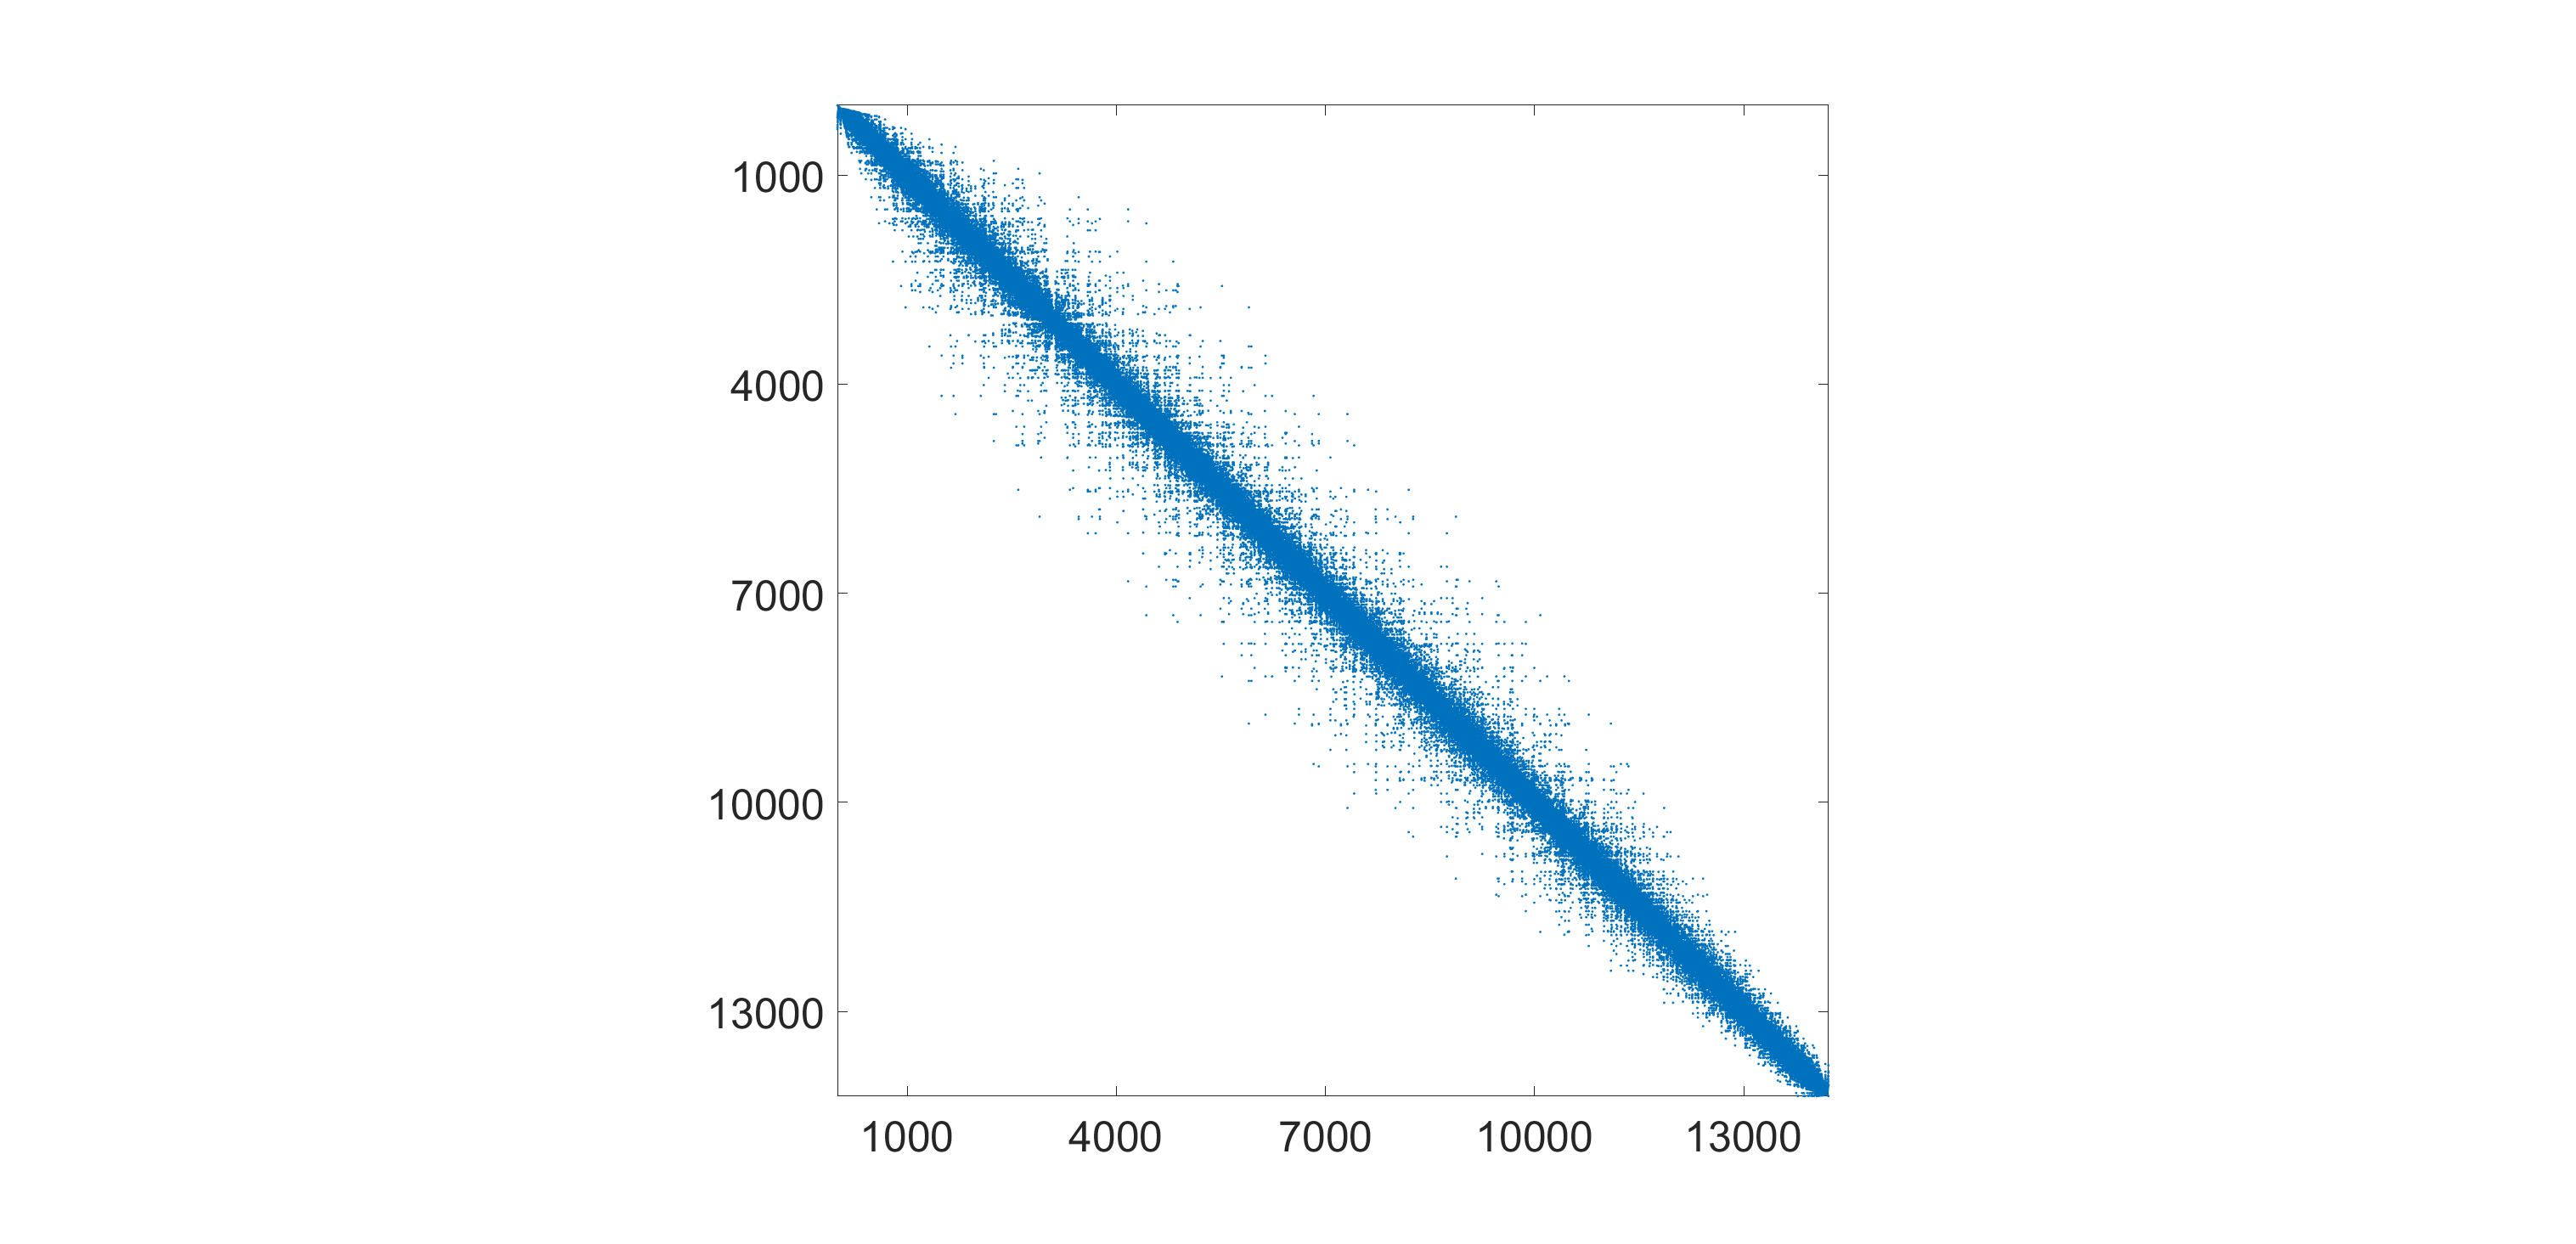
\includegraphics[width=\textwidth,trim={410 40 400 40},clip]{2d_airfoil.eps}
				\caption{}
				\label{fig:mat_foil}
			\end{subfigure}
			\enskip
			\begin{subfigure}{0.3\textwidth}
				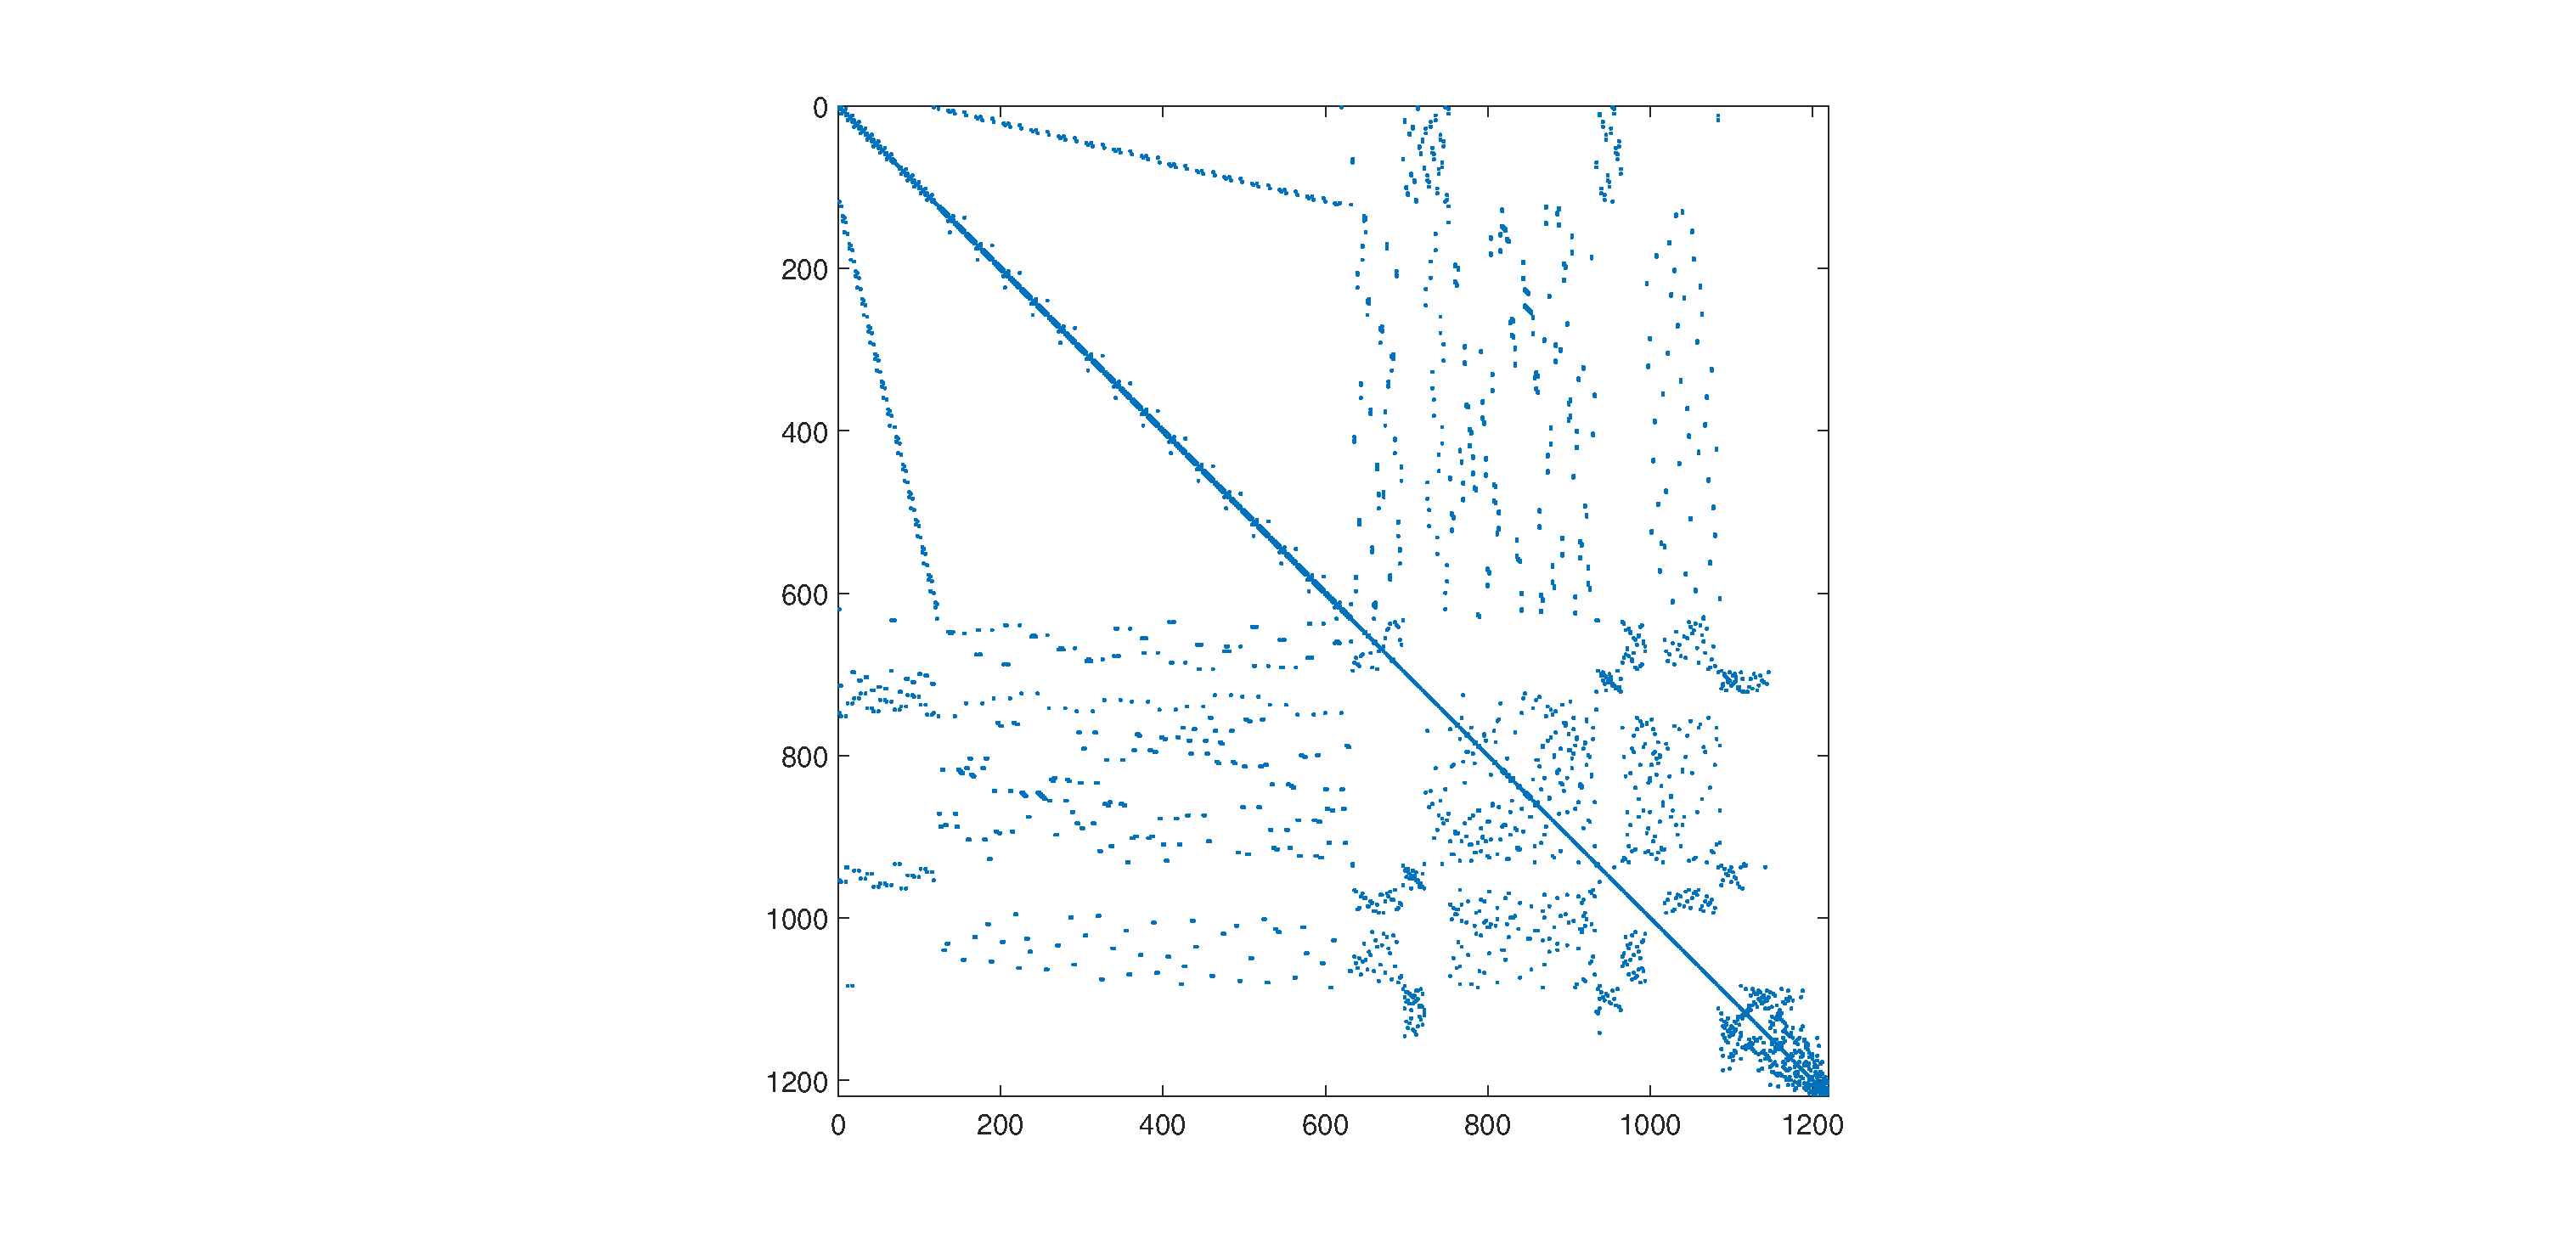
\includegraphics[width=\textwidth,trim={410 40 400 40},clip]{2d_fan.eps}
				\caption{}
				\label{fig:mat_fan}
			\end{subfigure}
			\caption{Stiffness matrices exhibiting different sparsity and non-zero patterns. The systems described by these matrices are \subref{fig:mat_beam} notched beam; \subref{fig:mat_foil} a laminar airfoil; \subref{fig:mat_fan} jet engine compressor fan.}
			\label{fig:matrices}
		\end{figure}
		
		\bibliographystyle{elsarticle-num}
		\bibliography{peter_bib}
		
\end{document}
